\thispagestyle{fancy}
\begin{center}
	\LARGE{\textbf{Ley de ohm (Primera parte)}}
\end{center}
\section{Objetivos}
Al finalizar esta experiencia, usted estará capacitado para:
\begin{enumerate}
	\item Demostrar la primera ley de Ohm en forma experimental.
	\item Determinar el valor de los resistores, a partir de los valores medidos de tensión y corriente.
	\item Determinar la corriente en un circuito a partir de la resistencia (determinada mediante el código de colores) y la tensión medida.
	\item Determinar la tensión en un circuito a partir de la resistencia (leída mediante el código de colores) y de la corriente medida con un amperímetro.
\end{enumerate}

\section{Conocimientos previos}
La ley de Ohm establece que la tensión en bornes de un resistor es igual al producto de su resistencia por la corriente que circula por el resistor.
Esta ley puede ser utilizada para cálculo de la tensión, corriente y la resistencia. 
Las ecuaciones son:
\begin{equation*}
	V=I*R 
\end{equation*}
\begin{equation*}
	I=V/R
\end{equation*}
\begin{equation*}
	R=V/I
\end{equation*}
Donde:
\begin{itemize}
	\item \textbf{V} tensión a través de resistor del resistor (en V)
	\item \textbf{I} corriente que circula por el resistor (en A) 
	\item \textbf{R} resistencia del resistor (en $\Omega $ )
\end{itemize}

\section{Autoevaluación}
\begin{enumerate}
	\item La corriente es proporcional a la tensión en bornes del resisto.r
	\item Si la tensión en los bornes de un resistor es $30 V$ y la corriente en el mismo vale $0.1A$, la resistencia vale $3k\Omega$.
\end{enumerate}

\section{Equipo}
El siguiente equipo es necesario para realizar la experiencia.
\begin{enumerate}
	\item Modulo de experimentos
	\item Uno o dos DMM (Multímetros)
\end{enumerate} 
\section{Procedimiento}
\begin{enumerate}
	\item Estudie e implemente el circuito de la figura 1
	\item Ajuste la fuente de alimentación PS-1 a su mínima tensión de salida. Conecte R1 y el multímetro a la fuente de alimentación del modo que se muestra a continuación.
	
	\begin{figure}[h]
		\centering
		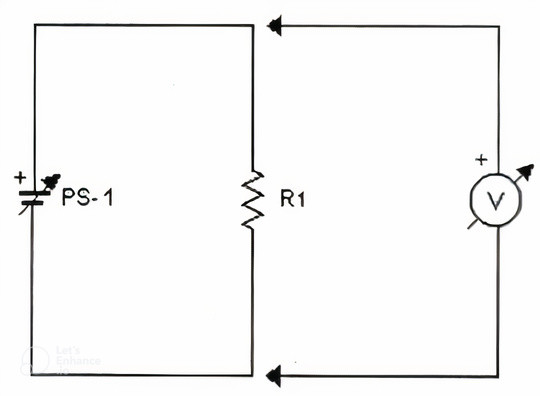
\includegraphics[scale=0.5]{imagenes/4.1}
		\caption{Circuito a armarse}
	\end{figure}
	\item Lleve el DMM al de medición de tensión continua, en la escala de 10 V. lleve la tensión en de CC a cero. Este es el primer valor en la cuadro 1.
	\\
\begin{table}[htbp]
	\centering
	
	\begin{tabular}{|c|c|c|}
		\hline
		\text{Tensión (V)} & \text{Corriente en R1 (mA)} & \text{Corriente en R2 (mA)} \\
		\hline
		0 & 0.1 & 3.3 \\
		\hline
		2& 0.4 &8.9 \\
		\hline
		4& 0.9 & 18.6 \\
		\hline
		6& 1.3 &27.5 \\
		\hline
		8& 1.7 & 37.3 \\
		\hline
		10& 2.1 & 47 \\
		\hline
	\end{tabular}
	\caption{Las resistencias usadas fueron $4.7K\Omega$ y $0.2K \Omega$ respectivamente}
\end{table}

		\item Retire el multímetro y ajústele para medir corrientes (escala de 20mA). Conecte el DMM para medir la corriente en R1 como se muestra en la figura 2.
		\\
		\\
		\\
		\\
		\\
		\\
		\\
		\\
		\begin{figure}[h]
			\begin{minipage}{0.4\textwidth}
				\centering
				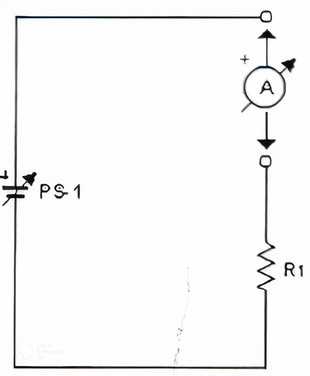
\includegraphics[width=\textwidth]{imagenes/4.2}
				\caption{Primera medición}
				\label{fig:imagen1}
			\end{minipage}%
			\begin{minipage}{0.5\textwidth}
				\centering
				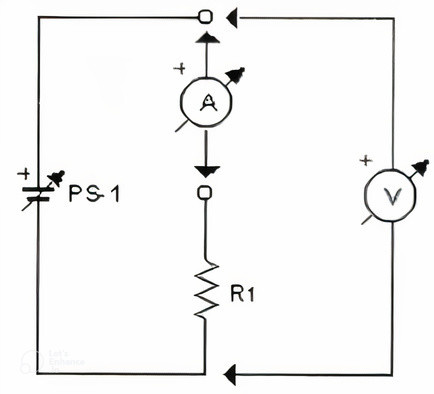
\includegraphics[width=\textwidth]{imagenes/4.3}
				\caption{Segunda medición}
				\label{fig:imagen2}
			\end{minipage}
		\end{figure}
		\\ \textbf{Nota:} si dispone de dos multímetros, use el primero para medir la tensión den bornes de R1 y el segundo como amperímetro figura 3.
		
		\item Repita el procedimiento: lleve la tensión de PS-1 el valor requerido, mida la corriente que circula por R1, y registre su valor en la cuadro 1.
		\item Repita el procedimiento de fijar la tensión y medir la corriente con R2 en lugar de R1 registre su valor en la cuadro 1.
		\item Repita el procedimiento de fijar la tensión y medir la corriente con R3 en lugar de R1, y registre su valor en la cuadro 1.
		\item En los pasos 3 a 6 se procedió  a variar la tensión en los bornes y anotando los valores de la corriente.\\
		Utilizando los resultados de la tabla cuadro 1 construya el grafico de la corriente (en el eje vertical), en la función de la tensión en bornes (en el eje horizontal). Muestre los tres conjuntos de resultados den el mismo grafico y denomínelos R1 y R2.
	\\
	\\
	\\
	\\
	\\
	\\
	\\
	\\
	\\
	\\
	\\
		
		\begin{figure}[h]
			\centering
			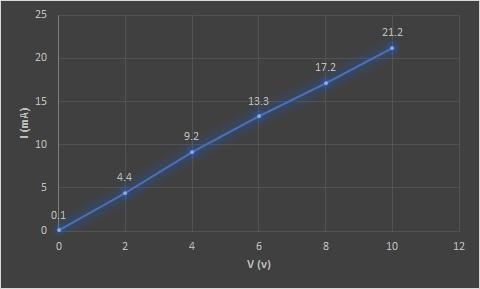
\includegraphics[scale=1]{imagenes/9.1}
			\caption{Gráfica de la resistencia $4.7k\Omega$}
		\end{figure}
		\begin{figure}[h]
			\centering
			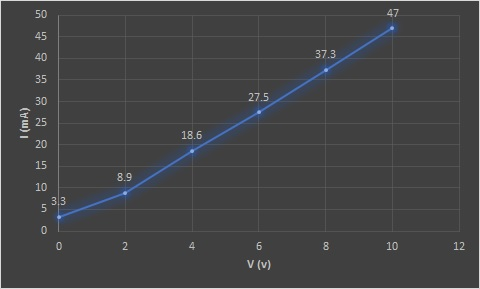
\includegraphics[scale=1]{imagenes/9.2}
			\caption{Gráfica de la resistencia $0.2k\Omega$}
		\end{figure}
	
		
		\item Utilizando la ecuación $I=V/R$ calcule la corriente que circula por cada resistor (cuyos valores son conocidos a partir del código de colores), y marque los puntos con un "X".
		\\
		\\
		\\
		\\
		\\
		\\
		\\
		\\
		\\
		\\
		\\
		\\
			\begin{figure}[h]
			\centering
			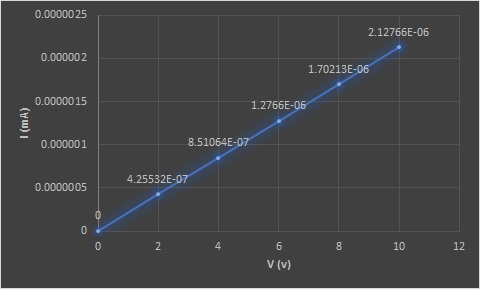
\includegraphics[scale=1]{imagenes/10.2}
			\caption{Gráfica de la resistencia $4.7k\Omega$}
		\end{figure}
		\begin{figure}[h]
			\centering
			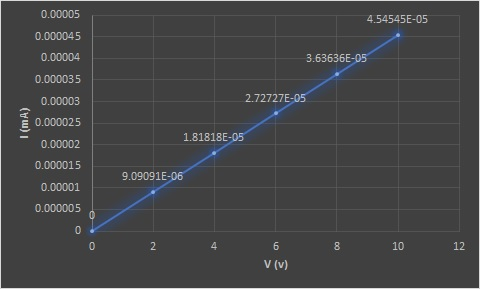
\includegraphics[scale=1]{imagenes/10.1}
			\caption{Gráfica de la resistencia $0.2k\Omega$}
		\end{figure}
	
	\end{enumerate}
\section{Conclusiones}
Con el laboratorio N°04, se llego a profundizar los conocimientos de la ley de Ohm ($\textbf{V=IR}$, $\textbf{I=V/R}$ y $\textbf{R=V/I}$), donde cuando las intensidades  y el valor de la resistencia suben, tensión medida en los resistores también suben; por lo tanto podemos afirmar que la el voltajes (V) es directamente proporcional al valor de las resistencias y de corriente. El valor de la corriente va depender de la división del voltaje (V) y resistencia ($\Omega$), si el valor del voltaje sube y la renitencia se mantiene con un valor inicial, entonces el valor de la corriente también sube; si el valor de la resistencia sube y el valor del voltaje se mantiene en ese caso el valor de la corriente disminuye. Lo mismo que ocurre para el valor de la corriente pasa para la resistencia, solo en este caso que la formula se invierte la es la división del voltaje entre la corriente.Para finalizar no siempre va ser igual los valores medido con el valor teórico  en las resistencias, puesto que existe un pequeño marguen de error y también las resistencias tienen una tolerancia de $10\%$ o $ 5\%$.
